% !TEX program = xelatex
% Compile with: xelatex report.tex
\documentclass[12pt,a4paper,oneside]{report}
\usepackage[utf8]{inputenc}
\usepackage{kotex}
\usepackage{amsmath,amssymb,amsthm}
\usepackage{graphicx}
\usepackage{float}
\usepackage[margin=1in, headheight=14.5pt]{geometry}
\graphicspath{{figures/}{attachments/}}
\usepackage{hyperref}
\usepackage{booktabs}
\usepackage{longtable}
\usepackage{array}
\usepackage{tabularx}
\usepackage{natbib}
\usepackage{setspace}
\usepackage{fancyhdr}
\usepackage{titlesec}
\usepackage{enumitem}
\usepackage{microtype}
\usepackage{xcolor}
\usepackage{caption}
\usepackage{multirow}
\usepackage{subcaption}
\usepackage{indentfirst}
\setlength{\parindent}{1em}

\hypersetup{
  colorlinks=true,
  linkcolor=blue!60!black,
  citecolor=green!50!black,
  urlcolor=blue!70!black
}

\titleformat{\chapter}[display]
  {\normalfont\huge\bfseries}{\chaptertitlename\ \thechapter}{18pt}{\Huge}
\titlespacing*{\chapter}{0pt}{-20pt}{30pt}

\pagestyle{fancy}
\fancyhf{}
\fancyhead[L]{\slshape\nouppercase{\leftmark}}
\fancyhead[R]{\thepage}
\renewcommand{\headrulewidth}{0.4pt}

\onehalfspacing

\newtheorem{theorem}{Theorem}[chapter]
\newtheorem{definition}[theorem]{Definition}
\newtheorem{proposition}[theorem]{Proposition}

\renewcommand{\tablename}{표}
\renewcommand{\figurename}{그림}
\renewcommand{\contentsname}{목\ 차}
\renewcommand{\bibname}{참고문헌}
\renewcommand{\appendixname}{부록}

\begin{document}

% ================================================================
% 표지
% ================================================================
\begin{titlepage}
\centering
\vspace*{2cm}
{\Huge\bfseries 다중객체추적 데이터 연관에서\\[0.3cm] 검출 불확실성은 활용 가능한가\par}
\vspace{1cm}
{\Large 네 가지 주입 경로 비교와 오라클 상한 분석\par}
\vspace{1cm}
{\large\itshape Is Detection Uncertainty Usable for Data Association \\ in Multi-Object Tracking? \\ A Controlled Comparison of Four Injection Channels\par}
\vfill
{\Large\bfseries 12241701 박준형\par}
\vspace{0.6cm}
{\large 인하대학교 데이터사이언스학과\par}
\vspace{1.2cm}
{\large 2026년\par}
\end{titlepage}

% ================================================================
% 요약
% ================================================================
\chapter*{요\ \ \ 약}
\addcontentsline{toc}{chapter}{요약}

다중객체추적(Multi-Object Tracking, MOT)의 데이터 연관은 트랙과 검출 사이의 비용 행렬을 만들고 헝가리안 알고리즘으로 푸는 방식이 표준이다. 이 비용에 검출기가 제공하는 \textbf{위치 불확실성}을 넣으면 성능이 개선될 것이라는 기대가 있어 왔으나, 보고된 결과는 일관되지 않는다. 본 연구는 이 기대를 MOT17 데이터에서 통제된 조건으로 검증한다.

동일한 검출 결과를 캐시로 고정하여 비교군 사이에서 비트 단위로 같게 유지한 상태에서, 검출 불확실성 $\sigma$를 네 가지 경로 --- 칼만 필터 측정잡음 $R$, 거리 함수, 게이팅(박스 확장), 매칭 임계값 --- 에 주입하고 HOTA로 평가하였다. 또한 $\sigma$의 두 가지 산출 방식(NMS 후보 분산, DFL 분포 분산)을 같은 절차로 비교하였다.

핵심 결과는 다음과 같다. 첫째, $\sigma$는 \textbf{위치 오차}를 예측한다 --- 박스 높이를 통제한 편상관계수 중앙값 $+0.322$이며 7개 시퀀스 전부에서 양의 값을 보였다. 둘째, 그럼에도 \textbf{밀도 모형으로는} 박스 크기 기반 모형에 7개 시퀀스 전부에서 패배하였다(양측 부호검정 $p = 0.0156$). 이는 자유도를 자유롭게 적합한 Student-$t$ 분포에서도 동일하였다. 단 이 패배는 NMS 후보 분산에 대한 것이며, DFL 분포 분산은 방향이 반대였다(6/7, $p = 0.125$로 유의성 미달). 셋째, 네 가지 주입 경로 모두 HOTA 기준 음의 결과를 보였다($-0.21 \sim -4.98$). 넷째, 그 원인을 규명하기 위해 \textbf{연관 오라클 상한}을 측정한 결과 이 데이터에서 데이터 연관이 개선할 수 있는 최대치는 $+3.122$ HOTA였으며, 개선 여지 자체는 존재하였다. 다섯째, 그 여지에 $\sigma$로 도달할 수 있는지를 직접 측정한 결과 \textbf{$\sigma$는 연관 오류를 예측하지 못하였다} --- 1단계 매칭에서 채택된 쌍 가운데 정답 여부를 판별할 수 있는 29{,}571쌍에 대한 AUC가 $0.4571$로 무작위 수준(0.5) 아래였고, 박스 높이를 통제한 편상관계수는 $-0.0220$이었다.

이 결과는 네 경로의 음의 결과가 ``주입 경로의 문제''가 아니라 \textbf{$\sigma$ 안에 연관 오류에 대한 정보가 없기 때문}임을 시사한다. 박스 크기 기반 $\sigma_C$ 역시 AUC $0.4661$로 예측력이 없었으므로, 이는 특정 산출 방식의 문제가 아니라 검출 품질 신호 전반의 한계로 해석된다. 부수적으로 본 연구는 검출별 스칼라를 비용에 \textbf{덧셈}으로 넣으면 최적 할당이 바뀌지 않음을 실제 데이터에서 확인하였으며(불일치 12건 전부 동점, 최적성 위배 0건), 이는 문헌이 예외 없이 곱셈 형태를 사용해 온 사실에 대한 설명을 제공한다.

\vspace{0.3cm}
\noindent\textit{핵심어: 다중객체추적, 데이터 연관, 검출 불확실성, 오라클 상한, 음의 결과, 사전 등록}

\vspace{0.2cm}
\noindent 본 연구는 사전 등록된 실험 계획, 재현 가능한 캐시 기반 실험 설계, 그리고 15건의 철회 기록을 함께 공개한다. 코드와 실험 기록은 \url{https://github.com/JunHyeong-data/mot-assoc}에서 확인할 수 있다.

% ================================================================
% 목차
% ================================================================
\tableofcontents

% ================================================================
% Ⅰ. 서론
% ================================================================
\chapter{서론}

다중객체추적은 매 프레임에서 검출된 객체를 기존 트랙에 연결하는 작업이다. 표준적인 접근인 tracking-by-detection 방식에서 이 연결은 트랙 $M$개와 검출 $N$개 사이의 비용 행렬을 구성하고 헝가리안 알고리즘\citep{kuhn1955}으로 최적 할당을 구하는 방식으로 이루어진다. SORT\citep{bewley2016}는 이 비용으로 IoU를 사용하였고, DeepSORT\citep{wojke2017}는 마할라노비스 거리와 외형 특징을 결합하였으며, ByteTrack\citep{zhang2022}은 IoU를 유지하되 낮은 점수의 검출까지 2단계로 활용하였다.

이 비용 행렬에 \textbf{검출기가 제공하는 위치 불확실성}을 반영하면 성능이 개선되리라는 기대는 자연스럽다. 검출기가 어떤 박스의 위치를 확신하지 못한다면, 그 정보는 연관 판단에 유용해야 한다는 직관이다. 실제로 이 방향의 시도가 여럿 있었다. UTrack\citep{solano2024}은 NMS 후보들의 분산을 검출 불확실성으로 삼아 칼만 필터에 전파하였고, UncertaintyTrack\citep{lee2024}은 검출기가 직접 예측한 공분산을 사용하였다.

그러나 보고된 결과는 기대와 다르다. UncertaintyTrack의 저자들은 자신들의 절제 실험에서 칼만 필터 측정잡음 교체가 \textit{단독으로는 성능을 떨어뜨린다}고 명시하였으며, 그 원인에 대해 다음과 같이 기술하였다.

\begin{quote}
``It is possible that the multivariate Gaussian distribution does not accurately represent the true underlying uncertainty distribution, suggesting that the uncertainty estimates might not be compatible with the Kalman Filter. \textit{This remains an area for future investigation.}''\citep{lee2024}
\end{quote}

즉 원인은 \textbf{추측으로 남아 있다}. 본 연구는 이 자리에 측정값을 넣는 것을 목표로 한다.

주목할 점은 이 문제가 최근에 제기된 것이 아니라는 사실이다. DeepSORT는 2017년에 이미 매칭 캐스케이드를 도입하면서 그 동기를 다음과 같이 밝혔다.

\begin{quote}
``When two tracks compete for the same detection, the Mahalanobis distance favors larger uncertainty $\ldots$ This is an undesired behavior as it can lead to increased track fragmentations and unstable tracks.''\citep{wojke2017}
\end{quote}

이는 본 연구가 \textbf{공분산 역설}이라 부르는 현상 --- 불확실성이 클수록 마할라노비스 거리가 작아져 오히려 선호되는 구조 --- 을 정확히 지적한 것이다. DeepSORT는 이를 비용 함수를 수정하는 대신 트랙 나이 순서의 캐스케이드로 \textbf{우회}하였다. 이후 UCMCTrack\citep{yi2024}이 거리에 로그 행렬식 항을 더해 이 편향을 \textbf{억제}하는 방법을 제시하였다(2.5절). 그러나 두 대응 모두 \textbf{불확실성을 무엇으로 재는가는 건드리지 않는다} --- 전자는 순서로 피해 가고, 후자는 벌점을 더할 뿐이다. \textbf{검출기가 산출한 불확실성이 연관에 쓸모가 있는지 자체를 통제된 조건에서 측정한 연구는 찾기 어렵다.}

본 연구의 목적은 다음 세 가지이다.

첫째, \textbf{검출 불확실성이 데이터 연관에 도달하는지를 통제된 조건에서 측정한다.} 검출 결과를 캐시로 고정하여 비교군 사이에서 완전히 동일하게 유지하고, 주입 경로만을 변화시켜 그 효과를 분리한다.

둘째, \textbf{음의 결과가 나올 경우 그 원인을 규명한다.} ``주입 경로가 부적절해서''인지 ``애초에 개선할 여지가 없어서''인지 ``$\sigma$ 안에 정보가 없어서''인지는 서로 다른 주장이며, 이를 구별하기 위해 연관 오라클 상한을 측정하는 방법을 도입한다.

셋째, \textbf{설계 제약을 실제 데이터에서 확인한다.} 검출별 스칼라를 비용에 어떤 형태로 넣어야 하는지에 대한 이론적 제약을 유도하고, 이를 실측으로 검증한다.

논문의 구성은 다음과 같다. 2장에서 관련 연구를 검토하고 신호의 산출 방식과 주입 경로라는 두 축으로 정리한다. 3장에서 데이터와 실험 환경을 기술하며, 4장에서 설계 제약과 비교 방법, 평가지표를 정의한다. 5장에서 실험 결과를 검출 수준과 추적 수준으로 나누어 제시하고, 6장에서 원인을 분석한다. 7장에서 결론과 한계를 논의한다.

% ================================================================
% Ⅱ. 관련 연구
% ================================================================
\chapter{관련 연구}

\section{신호의 산출 방식과 주입 경로}

검출 불확실성을 데이터 연관에 활용하는 연구는 두 가지 축으로 정리할 수 있다. 하나는 \textbf{신호를 어디서 얻는가}(산출 방식)이고, 다른 하나는 \textbf{그 신호를 어디에 넣는가}(주입 경로)이다. 본 연구는 이 두 축을 분리하여 보는 것이 문헌의 성패를 이해하는 데 핵심이라고 본다. 그림~\ref{fig:map}에 주요 방법들의 위치와 보고된 결과를 정리하였다.

\begin{figure}[htbp]
\centering
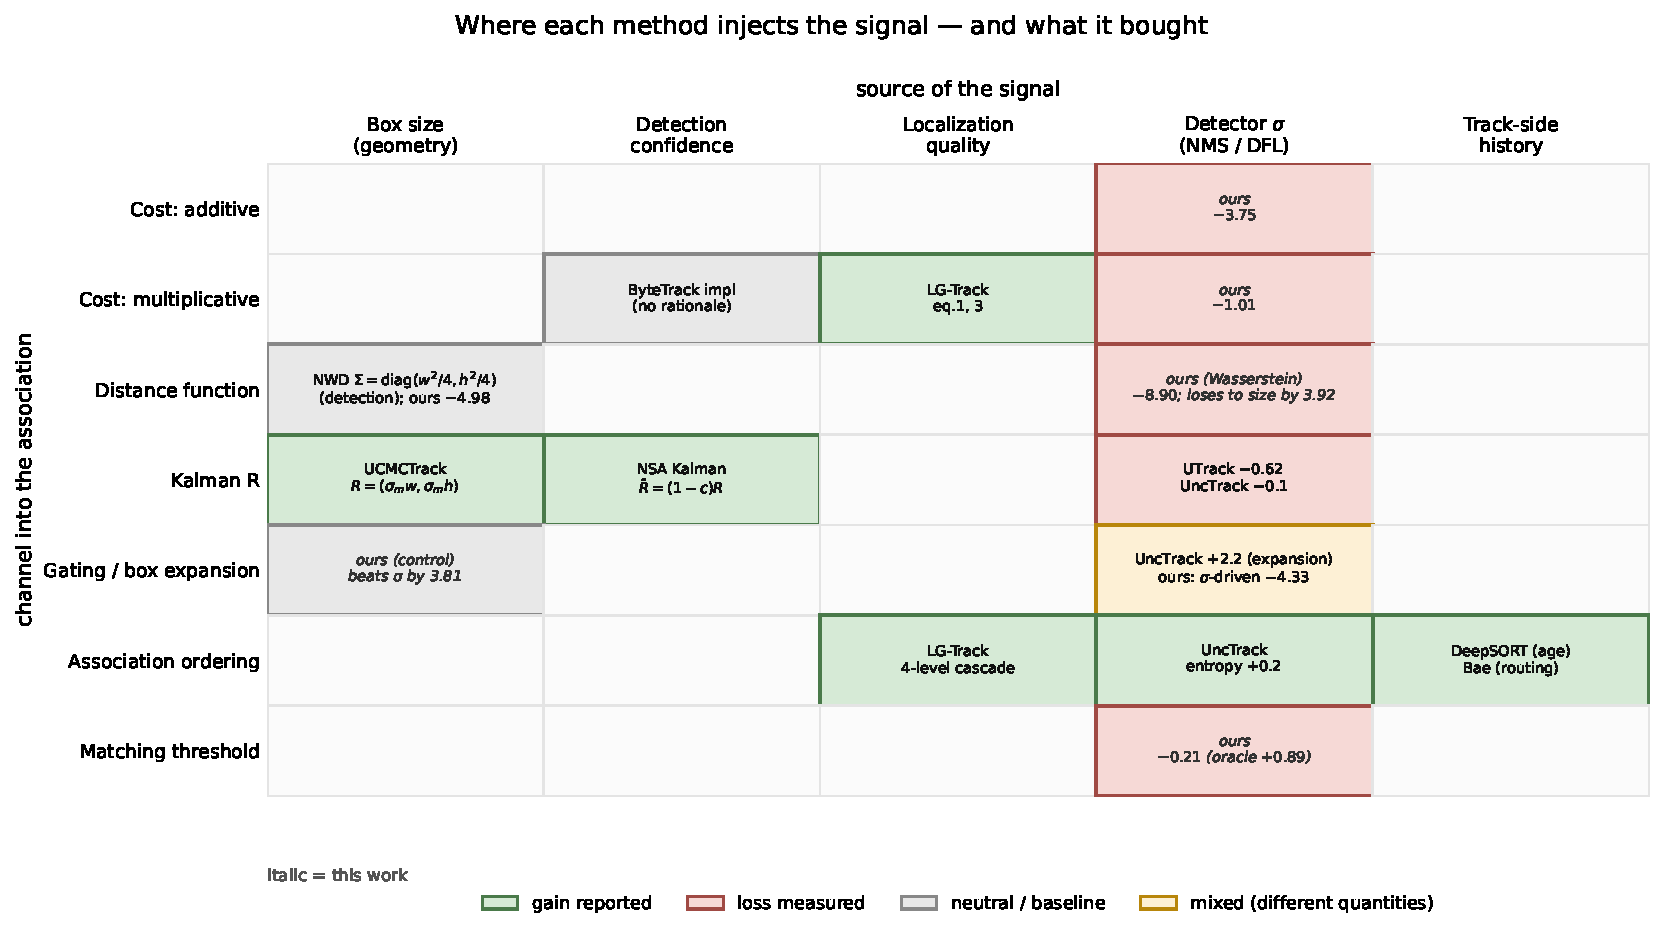
\includegraphics[width=\textwidth]{figures/fig_source_channel.pdf}
\caption{신호의 산출 방식(가로축) $\times$ 주입 경로(세로축) 지도. 각 칸은 해당 조합을 사용한 방법과 보고된 결과를 나타낸다. 기울임체는 본 연구의 결과이다. 모든 항목은 원문을 직접 확인하여 작성하였다.}
\label{fig:map}
\end{figure}

\section{산출 방식: 무엇을 불확실성으로 삼는가}

\paragraph{박스 크기 기반} 가장 널리 쓰이는 방식은 박스의 폭과 높이에 비례하는 공분산을 가정하는 것이다. NWD\citep{wang2021}는 바운딩 박스를 2차원 가우시안으로 모형화하며 $\Sigma = \mathrm{diag}(w^2/4,\, h^2/4)$를 사용한다. UCMCTrack\citep{yi2024}은 칼만 필터의 측정잡음을 $R_{uv} = \mathrm{diag}((\sigma_m w)^2,\, (\sigma_m h)^2)$로 정의하는데, 여기서 $\sigma_m$은 하이퍼파라미터이고 $w, h$는 검출된 박스의 폭과 높이이다. 즉 이 방식은 검출기가 산출한 불확실성이 아니라 \textbf{기하학적 크기}를 대리 변수로 사용한다.

\paragraph{검출 신뢰도 기반} NSA Kalman\citep{du2023}은 검출 신뢰도 $c$를 이용해 측정잡음을 $\tilde{R} = (1-c) R$로 조정한다. 신뢰도가 높을수록 잡음을 작게 보는 직관적 규칙이다.

\paragraph{검출기 산출 불확실성} UTrack\citep{solano2024}은 NMS 과정에서 억제된 후보 박스들의 중심 분산을 불확실성으로 사용한다. 검출기 구조를 변경하지 않고 추론 이후에 측정한다는 점이 설계 의도이다. UncertaintyTrack\citep{lee2024}은 검출기가 직접 분포 매개변수를 예측하도록 학습시킨다. GFLv2\citep{li2021}는 검출 단계에서 DFL(Distribution Focal Loss) 분포의 통계량(상위 4개 값과 평균)으로 위치 품질을 예측하였으나, 추적으로 확장하지는 않았다.

\section{주입 경로: 어디에 넣는가}

\paragraph{칼만 필터 측정잡음} 가장 많이 시도된 경로이다. 위에서 언급한 UCMCTrack, NSA Kalman, UTrack, UncertaintyTrack이 모두 여기에 해당한다. \textbf{같은 경로임에도 결과가 갈린다는 점이 중요하다} --- 박스 크기를 사용한 UCMCTrack은 SOTA를 달성한 반면, 검출기 산출 불확실성을 사용한 두 연구는 손실을 보고하였다.

\paragraph{거리 함수} IoU를 분포 간 거리로 대체하는 접근이다. NWD가 대표적이며, UCMCTrack은 정규화된 마할라노비스 거리 $D = \epsilon^\top S^{-1} \epsilon + \ln|S|$를 사용한다. 여기서 로그 행렬식 항은 공분산 역설을 억제하기 위한 것으로, 저자들은 그 목적을 ``측정의 정확도와 불확실성까지 함께 고려하기 위해''라고 명시하였다.

\paragraph{게이팅과 박스 확장} UncertaintyTrack의 절제 실험에서 \textbf{가장 큰 기여}를 보인 성분이다(mMOTA $+2.2$, mIDF1 $+3.0$). 불확실성에 비례하여 박스를 키워 겹침 확률을 높이는 방식이다.

\paragraph{연관 순서와 라우팅} DeepSORT는 트랙 나이 순으로 캐스케이드를 구성하고, Bae와 Yoon\citep{bae2014}은 tracklet confidence로 지역 연관과 전역 연관을 분기한다. 두 방식 모두 \textbf{트랙 쪽} 양을 사용한다. 검출 쪽 신호를 사용한 사례로는 LG-Track\citep{meng2023}의 4단계 캐스케이드와 UncertaintyTrack의 엔트로피 기반 그리디 매칭이 있다.

\section{비용 함수의 형태에 대한 관찰}

원문을 검토한 결과 한 가지 규칙성이 관찰된다. \textbf{문헌이 검출별 스칼라를 비용에 넣을 때는 예외 없이 곱셈 형태를 사용한다.} LG-Track은 $C_1 = C_{\mathrm{iou}} \cdot d_l$, $C_3 = C_{\cos} \cdot d_s$의 형태를 사용하고, ByteTrack 구현체는 $\mathrm{cost} = 1 - \mathrm{IoU} \cdot s$를 사용한다. 덧셈 형태를 사용한 사례는 찾을 수 없었다.

주목할 점은 \textbf{이 형태를 선택한 이유를 밝힌 문헌이 없다}는 것이다. 특히 ByteTrack의 경우, 본 연구가 논문 전문(64{,}480자)을 검색한 결과 점수를 비용에 곱하는 식이 \textbf{논문에 존재하지 않는다}. 논문에서 검출 점수는 높음과 낮음을 나누는 기준으로만 사용되며, 유사도는 ``IoU 또는 Re-ID 특징 거리''로 기술된다. $\mathrm{cost} = 1 - \mathrm{IoU} \cdot s$는 구현체에만 존재하는 설계이다. 4.1절에서 이 형태가 왜 필연적인지에 대한 설명을 제시한다.

\section{공분산 역설에 대한 기존 대응}

가림(occlusion) 구간에서 트랙의 공분산이 커지면 마할라노비스 거리가 작아져 오히려 매칭이 선호되는 현상이 발생한다. 이에 대한 대응은 세 갈래로 나뉜다. DeepSORT는 캐스케이드로 우회하였고, UCMCTrack은 로그 행렬식 항을 추가하여 억제하였다. OC-SORT\citep{cao2023}는 다른 문제를 다룬다 --- 관측이 없는 동안 상태 추정의 오차가 시간에 따라 증폭되는 현상(temporal error magnification)에 대응하며, 논문 본문에서 ``uncertainty''라는 용어를 사용하지 않는다. 즉 가림 구간에서 발생하는 두 가지 실패 --- \textbf{평균의 표류}와 \textbf{공분산의 팽창} --- 중 전자를 다룬 것이다.

% ================================================================
% Ⅲ. 데이터 및 실험 환경
% ================================================================
\chapter{데이터 및 실험 환경}

\section{데이터}

실험에는 MOT17\citep{milan2016} 학습 분할의 7개 시퀀스를 사용하였다. 각 시퀀스의 후반부 절반을 검증용으로 분리하는 \texttt{val\_half} 방식을 따랐으며, 이는 UTrack의 재현 실험과 조건을 맞추기 위한 선택이다. 시퀀스별 특성은 표~\ref{tab:seqs}와 같다.

\begin{table}[htbp]
\centering
\small
\caption{MOT17 val\_half 시퀀스 특성. 카메라 움직임은 연속 프레임에서 동일 객체 중심 이동의 중앙값이다.}
\label{tab:seqs}
\begin{tabular}{lrrrrr}
\toprule
\textbf{시퀀스} & \textbf{fps} & \textbf{해상도} & \textbf{프레임당 객체} & \textbf{카메라 움직임(px)} & \textbf{연속 IoU} \\
\midrule
MOT17-02 & 30 & $1920{\times}1080$ & 33.0 & 0.00 & 0.985 \\
MOT17-04 & 30 & $1920{\times}1080$ & 46.1 & 0.00 & 0.986 \\
MOT17-05 & 14 & $640{\times}480$   &  8.0 & 2.92 & 0.890 \\
MOT17-09 & 30 & $1920{\times}1080$ & 11.0 & 3.50 & 0.923 \\
MOT17-10 & 30 & $1920{\times}1080$ & 18.2 & 2.00 & 0.886 \\
MOT17-11 & 30 & $1920{\times}1080$ & 10.1 & 3.20 & 0.936 \\
\textbf{MOT17-13} & 25 & $1920{\times}1080$ &  8.4 & \textbf{9.22} & \textbf{0.572} \\
\bottomrule
\end{tabular}
\end{table}

MOT17-13은 카메라 움직임이 나머지의 약 3.8배로 두드러진다. 이 시퀀스는 이후 여러 지표에서 특이값을 보이므로 6.3절에서 별도로 분석한다.

\section{검출 결과의 고정}

본 연구의 핵심 통제는 \textbf{모든 비교군이 완전히 동일한 검출 결과를 사용하도록 만드는 것}이다. 검출기를 매번 실행하면 조건 간 차이에 검출 변동이 섞이게 되므로, 검출 결과를 한 번 산출하여 \texttt{npz} 파일로 저장하고 이후 모든 실험이 이를 재생하는 방식을 택하였다.

검출기는 UTrack이 공개한 가중치(\texttt{ablation\_17\_best.pt})를 사용하였고, 입력 크기 $800{\times}1440$, 신뢰도 임계값 0.01, NMS IoU 0.70으로 고정하였다. 7개 시퀀스의 val\_half 구간은 합계 2{,}652 프레임이며, 산출된 검출은 합계 63{,}137건이다.

이 설계의 이점은 두 가지이다. 첫째, 조건 간 검출이 비트 단위로 동일하므로 성능 차이를 연관 방식의 차이로 온전히 귀속할 수 있다. 둘째, 추적기 재생이 결정적이므로 실행 간 변동이 존재하지 않는다. 실제로 동일 조건을 처음부터 다시 재생하여 출력 파일의 해시를 대조한 결과 7개 시퀀스 전부에서 비트 단위로 일치하였다.

\section{추적기와 알려진 구현 문제}

추적기는 \texttt{ultralytics} 8.4.46의 ByteTrack 구현을 사용하고, 1단계 연관의 비용 계산 부분만 교체하였다. 이 구현에는 알려진 문제가 있다. 2단계 연관에서 \texttt{fuse\_score}가 적용되어 비용이 $1 - \mathrm{IoU} \cdot s$가 되는데, 2단계 검출은 정의상 $s < 0.25$이므로 비용이 항상 $0.75$를 초과한다. 그런데 2단계의 임계값은 $0.5$로 고정되어 있어 \textbf{어떤 쌍도 매칭될 수 없다}. 이 문제는 상류 저장소에서 2026년 7월에 독립적으로 발견되어 수정되었다.

본 연구는 이 문제의 영향을 직접 측정하였다. 2단계에서만 \texttt{fuse\_score}를 비활성화하여 참조 구현과 동일하게 만든 결과, 2단계 매칭이 0건에서 782건으로 살아났고 기준선 HOTA가 $-0.324$ 변화하였다. 이는 이후 제시할 추적 수준 결과($-0.21 \sim -4.98$)보다 한 자릿수 작은 크기이므로 결론을 뒤집지 않으나, 본 연구의 기준선을 문헌의 ByteTrack과 동일시할 수 없다는 점은 한계로 명시한다.

\section{검출 불확실성의 산출}

두 가지 산출 방식을 비교한다.

\paragraph{NMS 후보 분산} NMS 과정에서 특정 박스에 의해 억제된 후보들의 중심 좌표 공분산을 사용한다. UTrack의 방식과 동일하다. 구현 시 두 가지 함정이 있다. 첫째, NMS 함수는 입력 텐서를 제자리에서 변환하므로 호출 이전에 복사해야 한다. 둘째, letterbox 좌표와 원본 좌표가 다르며 좌표 변환이 NMS 이후에 적용되므로, 배율을 NMS 내부에서 측정하면 항상 정확히 1.0이 산출된다. 본 연구는 이 두 함정을 각각 겪었으며 그로 인한 잘못된 결론을 철회한 바 있다.

\paragraph{DFL 분포 분산} YOLOv8 계열의 검출 헤드는 박스의 각 변까지의 거리를 16개 구간의 분포로 예측하고 그 기댓값만 사용한다. 본 연구는 버려지는 \textbf{분산}을 불확실성으로 사용한다. 추가 추론 비용이 없다는 장점이 있다. 다만 이 방식은 DFL을 사용하는 검출기 계열에만 적용 가능하다.

\section{탐색적 분석: $\sigma$의 스케일 특성}

모델에 적용하기 전에 $\sigma$가 실제 위치 오차와 어떤 관계인지 확인하였다. 검출된 박스 중심과 대응하는 정답 박스 중심의 오차를 $\epsilon$이라 할 때, $z^2 = \epsilon^\top \Sigma_d^{-1} \epsilon$은 $\Sigma_d$가 올바른 공분산이라면 자유도 2의 카이제곱 분포를 따라야 한다.

측정 결과 $z^2$의 중앙값은 카이제곱 분포의 이론값 대비 \textbf{80배에서 562배}였으며(두 검출기 기준), 이는 $\sigma$가 실제 오차 대비 크게 과소 추정되어 있음을 의미한다. 더 중요한 것은 이 배율이 \textbf{시퀀스마다 크게 다르다}는 점이다(62배$\sim$1840배). 즉 단일 상수를 곱하는 방식의 보정으로는 충분하지 않다.

분포의 형태 또한 가우시안과 거리가 있다. 99\% 분위수를 50\% 분위수로 나눈 비율이 가우시안이라면 약 1.0이어야 하나 실측값은 \textbf{12에서 213}이었다. 이는 오차 분포의 꼬리가 매우 두껍다는 뜻이다.

% ================================================================
% Ⅳ. 방법론
% ================================================================
\chapter{방법론}

\section{설계 제약: 덧셈은 할당에 영향을 주지 않는다}

검출 불확실성을 비용에 반영하는 가장 단순한 방법은 검출별 스칼라를 더하는 것이다. 그러나 이 형태는 원리적으로 작동하지 않는다.

비용 행렬을 $C = [c_{ij}]$ ($i$는 트랙, $j$는 검출)라 하고, 검출별 스칼라 $u_j$를 더한 행렬을 $C' = [c_{ij} + u_j]$라 하자. 모든 실행 가능한 할당이 각 검출을 최대 한 번씩 사용하고, 검출 수가 트랙 수 이하($N \le M$)라면 모든 검출이 정확히 한 번씩 할당되므로 임의의 할당 $\pi$에 대해
\begin{equation}
\sum_{j} c'_{\pi(j)j} = \sum_{j} c_{\pi(j)j} + \sum_{j} u_j
\label{eq:col_const}
\end{equation}
가 성립한다. 식~(\ref{eq:col_const}) 우변의 두 번째 항은 $\pi$에 의존하지 않는 상수이므로 최적 할당은 변하지 않는다.

\begin{proposition}[검출별 스칼라의 가산 무효성]
$N \le M$인 할당 문제에서, 검출에만 의존하는 항을 비용에 더하는 것은 최적 할당을 변화시키지 않는다.
\end{proposition}

이는 헝가리안 알고리즘의 축소 단계가 근거하는 표준적 성질이며 새로운 정리가 아니다. 다만 본 연구가 강조하는 것은 이 성질의 \textbf{설계적 함의}이다.

\paragraph{따라서 불확실성은 트랙과 상호작용하는 형태로 들어가야 한다.} 곱셈 형태 $c_{ij} \cdot u_j$는 $c_{ij}$가 쌍에 의존하므로 이 제약을 피한다. 2.4절에서 관찰한 바와 같이 문헌은 예외 없이 곱셈을 사용해 왔으며, 본 관찰은 그 선택에 대한 설명을 제공한다.

\paragraph{덧셈을 쓰는 문헌이 반례가 아닌 이유} 비용에 항을 더하는 방법이 없는 것은 아니다. OC-SORT\citep{cao2023}의 OCM은 방향 일관성 항을 비용에 더한다. 그러나 이 항은 \textbf{트랙의 진행 방향과 검출의 위치에 함께 의존하는 쌍 항}이므로 검출별 스칼라가 아니고, 따라서 식~(\ref{eq:col_const})의 조건에 해당하지 않는다. 위 명제가 배제하는 것은 \textbf{검출에만 의존하는 항}이며, 쌍에 의존하는 항은 덧셈으로도 할당에 도달한다.

\paragraph{단, 임계값 경로는 예외이다.} 실제 추적기는 헝가리안 해를 구한 뒤 비용이 임계값을 넘는 쌍을 제거한다. 이 단계에서는 상수항도 채택 여부를 바꿀 수 있다. 즉 \textbf{할당에는 영향이 없으면서 결과는 바뀔 수 있으며}, 이 경우 성능 변화를 ``정보가 전달되었다''는 근거로 사용해서는 안 된다. 5.4절에서 이를 실측으로 확인한다.

\section{비교 조건}

$\sigma$를 네 가지 경로에 주입하고 각각을 기준선과 비교한다.

\begin{itemize}[leftmargin=2em]
\item \textbf{칼만 필터 측정잡음}: 트랙 상태 갱신 시 $R$을 검출별 $\sigma$로 대체. UTrack의 방식을 재현.
\item \textbf{거리 함수}: IoU를 2-Wasserstein 거리로 대체. 트랙과 검출을 각각 가우시안으로 보고 $W^2 = \|\epsilon\|^2 + \mathrm{tr}(\Sigma_t + \Sigma_d - 2(\Sigma_t^{1/2}\Sigma_d\Sigma_t^{1/2})^{1/2})$를 계산.
\item \textbf{게이팅(박스 확장)}: $\sigma$에 비례하여 박스를 확장한 뒤 IoU 계산.
\item \textbf{매칭 임계값}: 장면별로 임계값을 조정. $\sigma$를 포함한 장면 관측량으로 예측.
\end{itemize}

\paragraph{공정 비교를 위한 통제} 거리 함수를 교체하면 비용의 분포 자체가 달라지므로, 임계값을 그대로 두면 채택률이 변한다. 이 경우 성능 차이가 ``거리 함수의 차이''인지 ``채택률의 차이''인지 구별할 수 없다. 따라서 각 조건의 스케일 상수를 \textbf{기준선과 채택률이 일치하도록} 이분법으로 조정하였다.

게이팅 경로에서는 별도의 대조군을 두었다. $\sigma$로 확장한 조건과 \textbf{동일한 총 확장량을 박스 크기에 비례하여 분배한} 조건을 비교하면, 성능 차이를 ``확장 자체의 효과''가 아니라 ``확장량을 무엇으로 정했는가''로 귀속할 수 있다.

\section{연관 오라클 상한}

음의 결과가 나왔을 때 ``주입 경로가 부적절했다''와 ``애초에 개선할 여지가 없었다''는 서로 다른 설명이다. 이를 구별하기 위해 본 연구는 \textbf{연관 오라클 상한}을 측정하는 방법을 도입한다.

검출 결과를 고정한 상태에서 1단계 연관의 비용을 다음과 같이 대체한다.
\begin{equation}
c_{ij} =
\begin{cases}
0, & \text{트랙 } i \text{와 검출 } j \text{의 정답 ID가 같은 경우}\\
10^6, & \text{그 외}
\end{cases}
\end{equation}
검출에는 정답 박스와 IoU 0.5 이상으로 대응되는 ID를 부여하고, 트랙은 생성 시점의 검출로부터 ID를 물려받는다. 검출, 트랙 관리, 2단계 및 3단계 연관은 모두 그대로 유지한다.

\begin{equation}
\text{개선 여지} = \text{HOTA}(\text{오라클 연관}) - \text{HOTA}(\text{기준선})
\end{equation}

이 값은 \textbf{어떤 연관 방법이든 이 데이터에서 얻을 수 있는 최대치}이다. 정답을 사용하므로 성능 주장이 아니라 데이터에 대한 측정이며, 따라서 표본 크기에 따른 검정력 문제가 발생하지 않는다.

\paragraph{이 상한이 완전하지 않은 점} 오탐 검출과 미검출은 연관으로 고칠 수 없으므로 그대로 두었고, \texttt{track\_buffer}를 초과하여 사라진 객체가 새 트랙으로 생성되는 것도 수정하지 않았다. 따라서 이는 \textbf{달성 가능한 상한}이며 이론적 최대치보다 보수적이다.

\section{$\sigma$가 연관 오류를 예측하는지에 대한 직접 측정}

오라클을 통해 어떤 연관 결정이 틀렸는지 알 수 있으므로, 주입 경로와 무관하게 다음을 직접 물을 수 있다. \textbf{$\sigma$가 연관 오류를 예측하는가?}

1단계 연관에서 실제로 채택된 (트랙, 검출) 쌍마다 다음과 같이 분류한다.

\begin{itemize}[leftmargin=2em]
\item \textbf{정답}: 트랙과 검출의 정답 ID가 일치
\item \textbf{오류(수정 가능)}: ID가 불일치하지만 \textit{올바른 검출이 그 단계에 존재}
\item \textbf{오류(수정 불가)}: ID가 불일치하고 올바른 검출이 없음(미검출)
\item \textbf{판별 불가}: 검출에 대응하는 정답이 없음(오탐)
\end{itemize}

이 중 \textbf{수정 가능한 오류만이 연관 방법이 다룰 수 있는 대상}이다. 평가지표로는 $\sigma$가 이 오류를 구별하는 AUC를 사용한다. 분석 단위가 쌍이고 표본이 수만 건이므로 표본 크기 문제가 없다.

\section{평가지표}

추적 성능은 HOTA\citep{luiten2021}로 평가한다. HOTA는 검출 정확도(DetA)와 연관 정확도(AssA)의 기하평균으로 정의되어 두 측면을 분리해 볼 수 있다는 장점이 있다. 본 연구는 연관을 다루므로 AssA의 변화를 함께 보고한다.

\paragraph{평가 코드의 구성} 시퀀스가 조용히 누락되는 문제를 방지하기 위해, 표준 평가 도구의 지표 클래스만 사용하고 데이터 적재는 직접 구현하였다. 이는 과거 실험에서 설정 파일의 헤더 누락으로 첫 시퀀스가 평가에서 빠져 결과가 $-0.43$에서 $-0.62$로 달라진 사례를 겪었기 때문이다. 다만 MOTChallenge의 전처리 절차(distractor 클래스에 매칭된 예측 제거 등)는 원본을 그대로 복제하였다.

\paragraph{통계적 판단 기준} 추적 수준 결과의 분석 단위는 \textbf{장면}이며 본 연구는 7개를 사용한다. 이 표본 크기에서 부호검정이 유의수준 0.05를 만족하는 유일한 경우는 7개 전부가 같은 방향인 경우이다($p = 0.0156$). 검출 수준 결과는 분석 단위가 검출이므로 표본이 수만 건이며 이러한 제약이 없다. 5장은 이 두 층위를 명시적으로 구분한다.

% ================================================================
% Ⅴ. 실험 및 결과
% ================================================================
\chapter{실험 및 결과}

\section{검출 수준: $\sigma$는 위치 오차를 예측한다}

먼저 $\sigma$가 위치 오차와 관계가 있는지 확인하였다. 박스 높이가 오차와 $\sigma$ 양쪽에 영향을 주므로 높이를 통제한 편상관계수를 사용하였다. 결과는 그림~\ref{fig:transfer}(a)와 같다.

\begin{figure}[htbp]
\centering

\includegraphics[width=\textwidth]{figures/fig_signal_transfer.pdf}
\caption{동일한 $\sigma$, 동일한 시퀀스, 서로 다른 평가 대상. (a) 위치 오차에 대해서는 7개 시퀀스 전부에서 양의 상관을 보인다. (b) 연관 오류에 대해서는 7개 시퀀스 전부에서 무작위 수준(0.5) 아래이다.}
\label{fig:transfer}
\end{figure}

NMS 후보 분산의 편상관계수 중앙값은 $+0.322$이며 범위는 $+0.235 \sim +0.453$으로 \textbf{7개 시퀀스 전부에서 양의 값}을 보였다. DFL 분포 분산은 중앙값 $+0.151$로 더 약하였다. 이 관계는 검출기를 바꾸어도 유지되었고(COCO 사전학습 가중치 $+0.322$, MOT 학습 가중치 $+0.315$), 입력 해상도를 네 단계로 바꾸어도 유지되었다($+0.308 \sim +0.359$).

\textbf{즉 $\sigma$에는 신호가 있다.} 어느 검출의 위치가 부정확한지에 대한 정보를 담고 있다.

\section{검출 수준: 그러나 NMS 후보 분산은 밀도 모형으로 쓸 수 없다}

다음으로 $\sigma$를 확률 모형으로 사용할 수 있는지 확인하였다. 검출별 공분산을 사용하는 모형(A)과 박스 크기에 비례하는 공분산을 사용하는 모형(C)을 같은 조건에서 비교하였다. \textbf{두 모형은 자유 매개변수의 개수가 동일하다}(스케일 $k$와 자유도 $\nu$).

공정성을 위해 두 모형에 \textbf{동일하게} Student-$t$ 분포족을 부여하였다. 모형 A에만 두꺼운 꼬리를 허용하면 꼬리의 유연성 덕분에 이기는 것이 당연하므로, 이는 실험의 타당성에 필수적인 통제이다. 결과는 표~\ref{tab:nll}과 같다.

\begin{table}[htbp]
\centering
\small
\caption{검출별 공분산 모형(A) 대 박스 크기 모형(C)의 held-out 음의 로그우도 비교. 값이 낮을수록 좋으며, 차이가 양수이면 C의 승리이다.}
\label{tab:nll}
\begin{tabular}{llrrr}
\toprule
\textbf{산출 방식} & \textbf{절차} & \textbf{C 승리} & \textbf{쌍별 차이 중앙값} & \textbf{양측 $p$} \\
\midrule
\multirow{2}{*}{NMS 후보 분산} & LOSO (7-fold) & \textbf{7/7} & $+0.560$ nats & \textbf{0.0156} \\
                              & 전역 적합      & \textbf{7/7} & $+0.543$ nats & \textbf{0.0156} \\
\midrule
\multirow{2}{*}{DFL 분포 분산} & LOSO (7-fold) & 1/7 & $-0.096$ nats & 0.125 \\
                              & 전역 적합      & 1/7 & $-0.144$ nats & 0.125 \\
\bottomrule
\end{tabular}
\end{table}

NMS 후보 분산은 \textbf{7개 시퀀스 전부에서} 박스 크기 모형에 패배하였다. 이는 leave-one-sequence-out(LOSO) 방식과 전역 적합 방식 두 절차에서 동일하게 관찰되었다.

두 절차를 모두 사용한 이유는 LOSO의 각 fold가 학습 데이터를 공유하여 서로 독립이 아니기 때문이다. 7개 fold가 각각 6개 시퀀스로 적합되므로 이웃 fold는 학습 데이터를 5개 공유하며, 7/7을 $1/128$로 계산하는 것은 반보수적이다. 전역 적합은 \textbf{두 모형의 매개변수 개수가 같다}는 점을 이용해 각각 전체 데이터로 한 번씩 적합한 뒤 시퀀스별로 평가하므로 과적합 비대칭 없이 fold 의존성을 제거한다. 두 절차가 같은 결과를 주었으므로 이 우려는 해소된다.

\paragraph{DFL 분포 분산은 방향이 반대이다} 같은 절차에서 DFL 분포 분산은 오히려 박스 크기 모형을 \textbf{7개 중 6개에서 이겼다}(LOSO $-0.096$ nats, 전역 적합 $-0.144$ nats). 다만 이 결과는 \textbf{유의성에 도달하지 못하며}(양측 $p = 0.125$) 효과 크기도 작다. 4.5절에서 기술한 바와 같이 n=7에서 유의해지는 유일한 경우는 만장일치이므로 6/7은 원리적으로 유의해질 수 없다. 따라서 이를 \textbf{양성 결과로 주장하지 않는다.} 그러나 방향이 두 절차에서 일관된다는 점은 기록해 둔다 --- 이는 \textbf{두 산출 방식의 성격이 정반대}임을 시사한다. NMS 후보 분산은 순위는 잘 매기지만(5.1절, $+0.322$) 모형으로 쓸 수 없고, DFL 분포 분산은 순위가 약한 대신($+0.151$) 모형으로는 낫다. \textbf{따라서 이 절의 부정적 결론은 NMS 후보 분산에 대한 것이며, 검출기 산출 불확실성 일반에 대한 것이 아니다.}

\paragraph{꼬리가 원인이 아니다} 모형 A의 적합된 자유도는 7개 fold 전부에서 격자의 하한값($\nu = 1$, 코시 분포)에 도달하였다. 이는 적합 과정이 코시보다 더 두꺼운 꼬리를 원했다는 뜻이며, 즉 \textbf{최대한의 유연성을 부여했음에도 패배}하였다. 3.5절에서 관찰한 두꺼운 꼬리(비율 12$\sim$213)는 사실이지만, 그것을 수용하는 분포족을 주어도 결론이 바뀌지 않는다.

\paragraph{스케일 보정도 답이 아니다} 컨포멀 예측을 이용해 스케일을 보정하면 held-out 커버리지가 10.5\%에서 \textbf{96.1\%}로 개선되어 목표치 95\%에 도달하였다. 즉 \textbf{스케일은 고칠 수 있다}. 그럼에도 박스 크기 모형과의 우열은 바뀌지 않았다. 문제가 스케일이 아니라는 뜻이다.

\section{추적 수준: 네 경로 모두 음의 결과}

$\sigma$를 네 가지 경로에 주입하고 HOTA를 측정한 결과는 표~\ref{tab:channels}와 같다.

\begin{table}[htbp]
\centering
\small
\caption{주입 경로별 결과. 모든 조건에서 검출은 비트 단위로 동일하다.}
\label{tab:channels}
\begin{tabular}{llrl}
\toprule
\textbf{주입 경로} & \textbf{비교 대상} & \textbf{$\Delta$HOTA} & \textbf{통제} \\
\midrule
칼만 필터 $R$ & 기준선 & $-0.62$ & 저자 코드 재현 \\
거리 함수 & 기준선 & $-4.98$ & 채택률 일치, 검출 동일 \\
게이팅(박스 확장) & 확장량 일치 대조군 & $-4.33$ & 총 확장량을 맞춘 대조 \\
매칭 임계값 & 기본값 & $-0.21$ & LOSO 예측 규칙 \\
\bottomrule
\end{tabular}
\end{table}

\paragraph{게이팅 경로의 대조군이 특히 중요하다} 박스 확장 자체는 거의 비용이 들지 않는다($-0.52$). 그런데 \textbf{확장량을 $\sigma$가 결정하도록 하면} $-4.33$이 된다. 동일한 총 확장량을 박스 크기에 비례해 분배한 대조군과 비교하면 $\sigma$ 기반 확장이 $3.81$ HOTA 열등하다. 즉 이 설정에서 박스 확장의 이득은 \textbf{불확실성이 아니라 기하학적 확장}에서 온다.

\paragraph{이것은 UncertaintyTrack에 대한 반증이 아니다} 같은 방향의 결과이지만 구조가 다르다. 그들은 확장한 박스를 \textbf{2차 통과}에서 GIoU로 사용하는 반면 본 연구는 1단계 IoU에 직접 적용하였다. 그들이 보고한 mMOTA $+2.2$에 대해 말하려면 \textbf{같은 구조로 다시 측정해야 한다.} 본 결과가 뒷받침하는 것은 \textbf{확장량을 무엇으로 정하는가를 통제하지 않으면 확장의 이득을 불확실성에 귀속할 수 없다}는 방법론적 주장이며, 그들의 수치가 틀렸다는 주장이 아니다.

\paragraph{임계값 경로에는 애초에 여지가 거의 없다} 전역 최적 임계값은 기본값 대비 $+0.037$에 불과하였다. 시퀀스별 최적값은 0.70$\sim$0.98로 갈리지만, \textbf{정답을 알고 시퀀스마다 최적값을 선택해도 상한이 $+0.892$}이다. 장면 관측량으로 예측하는 규칙은 $-0.207$이었다.

\section{덧셈과 곱셈의 실측 비교}

4.1절의 설계 제약을 실제 데이터에서 확인하였다. 매 연관 호출마다 기준선 비용, 검출별 스칼라를 더한 비용, 곱한 비용 세 가지를 나란히 풀어 비교하였다. 두 섭동의 평균 크기는 동일하게 맞추었다(평균 $|\Delta \mathrm{cost}| = 0.1998$). 결과는 표~\ref{tab:addmul}과 같다.

\begin{table}[htbp]
\centering
\small
\caption{검출별 스칼라의 가산과 곱셈 비교. 1단계 연관 호출 2{,}645건 기준.}
\label{tab:addmul}
\begin{tabular}{lrr}
\toprule
\textbf{항목} & \textbf{덧셈} & \textbf{곱셈} \\
\midrule
임계값 적용 전 할당 일치율 ($N \le M$, 2{,}614건) & 99.54\% & 96.06\% \\
임계값 적용 전 할당 일치율 ($N > M$, 31건) & 54.84\% & --- \\
\quad 불일치 중 최적성 위배 & \textbf{0건} & --- \\
임계값 적용 후 채택 쌍이 달라진 호출 & \textbf{65.41\%} & 32.85\% \\
최종 HOTA & $-3.750$ & $-1.014$ \\
\bottomrule
\end{tabular}
\end{table}

덧셈 조건에서 할당이 달라진 12건은 \textbf{전부 동점}이었다. 즉 기준선 비용 기준으로 두 할당의 총비용이 동일하며, 헝가리안 알고리즘이 동점 상황에서 어느 최적해를 반환할지 정하지 않기 때문에 발생한 차이이다. \textbf{최적성이 위배된 사례는 0건이다.} 명제가 실제 데이터에서 성립한다. 명제의 조건이 필요하다는 것도 확인된다 --- $N > M$인 31건에서는 일치율이 54.84\%로 떨어진다.

동시에 4.1절이 예고한 예외도 확인되었다. 할당은 사실상 변하지 않는데 \textbf{임계값 단계에서 65.41\%의 호출에서 채택 결과가 달라지고}, 최종 HOTA는 $-3.750$이 된다. \textbf{즉 기여는 0인데 해롭기만 하다.} 반면 곱셈은 할당의 96.06\%만 유지되어(전체 호출 기준 95.88\%) 실제로 할당에 도달하며, 성능 저하도 $-1.014$로 더 작다.

\section{개선 여지는 존재하는가}

네 경로가 모두 실패한 이유로 ``애초에 개선할 여지가 없었다''는 설명이 가능하다. 이를 확인하기 위해 4.3절의 연관 오라클 상한을 측정하였다. 결과는 표~\ref{tab:ceiling}과 같다.

\begin{table}[htbp]
\centering
\small
\caption{연관 오라클 상한. 검출을 고정하고 1단계 연관만 정답으로 해결한 결과이다.}
\label{tab:ceiling}
\begin{tabular}{lrrrr}
\toprule
\textbf{조건} & \textbf{HOTA} & \textbf{DetA} & \textbf{AssA} & \textbf{IDSW} \\
\midrule
기준선 (IoU) & 61.002 & 58.801 & 64.036 & 275 \\
\textbf{연관 오라클} & \textbf{64.124} & 60.034 & \textbf{69.113} & \textbf{211} \\
\midrule
\textbf{개선 여지} & \textbf{$+3.122$} & $+1.233$ & $+5.077$ & $-64$ \\
\bottomrule
\end{tabular}
\end{table}

\textbf{개선 여지는 $+3.122$ HOTA로 존재한다.} 우리가 시도한 네 경로는 모두 음의 값이었으므로, ``딸 것이 없었다''는 설명은 기각된다. 4.3절에서 언급한 대로 이 상한은 오탐과 미검출을 수정하지 않으므로 보수적인 값이다.

\paragraph{DetA가 함께 오르는 이유} 검출 캐시가 동일함에도 DetA가 $+1.233$ 변화한다. 오라클 연관은 정답 ID가 다른 검출과의 매칭을 거부하므로 출력되는 트랙 행이 12.4\% 감소하고, 제거된 것의 상당수가 오탐이기 때문이다. \textbf{HOTA의 DetA는 검출 자체가 아니라 추적기 출력의 검출 품질이며, 그 출력을 무엇으로 채울지는 연관이 결정한다.}

\paragraph{여지는 장면에 몰려 있다} 시퀀스별 개선 여지는 $+0.91$(MOT17-04)에서 $+12.17$(MOT17-13)까지 13배 이상 차이가 난다. 이는 6.3절에서 별도로 분석한다.

\section{$\sigma$는 그 여지에 도달할 수 있는가}

개선 여지가 존재한다면, 다음 질문은 $\sigma$로 그 여지에 도달할 수 있는가이다. 4.4절의 방법으로 직접 측정하였다. 채택된 쌍의 구성은 표~\ref{tab:pairs}, 예측력 측정 결과는 표~\ref{tab:auc}와 같다.

\begin{table}[htbp]
\centering
\small
\caption{1단계에서 채택된 연관 쌍의 구성 (총 47{,}194쌍)}
\label{tab:pairs}
\begin{tabular}{lrr}
\toprule
\textbf{분류} & \textbf{건수} & \textbf{비율} \\
\midrule
정답 & 27{,}734 & 58.77\% \\
\textbf{오류 (수정 가능)} & \textbf{1{,}837} & \textbf{3.89\%} \\
오류 (수정 불가, 미검출) & 1{,}952 & 4.14\% \\
판별 불가 (오탐) & 15{,}671 & 33.21\% \\
\bottomrule
\end{tabular}
\end{table}

연관 방법이 다룰 수 있는 오류는 전체의 3.89\%이며, 이는 5.5절의 개선 여지 $+3.122$와 부합하는 규모이다.

\begin{table}[htbp]
\centering
\small
\caption{$\sigma$가 수정 가능한 연관 오류를 예측하는가 (정답 27{,}734건 대 오류 1{,}837건)}
\label{tab:auc}
\begin{tabular}{lr}
\toprule
\textbf{지표} & \textbf{값} \\
\midrule
AUC ($\sigma \rightarrow$ 수정 가능한 오류) & \textbf{0.4571} \\
AUC (박스 크기 기반 $\sigma_C$) & 0.4661 \\
박스 높이를 통제한 편상관계수 & \textbf{$-0.0220$} \\
\midrule
(참고) 위치 오차에 대한 편상관계수 & $+0.322$ \\
\bottomrule
\end{tabular}
\end{table}

\textbf{AUC가 0.5 미만이다.} 정보가 없는 정도가 아니라 미세하게 반대 방향이며, 시퀀스별로 보아도 $0.330 \sim 0.485$로 \textbf{7개 전부가 0.5 아래}이다(그림~\ref{fig:transfer}(b)). 위치 오차에 대한 편상관계수 $+0.322$와 나란히 놓으면 의미가 분명해진다.

\begin{quote}
\textbf{$\sigma$는 어느 박스의 위치가 틀렸는지는 알려주지만, 어느 짝짓기가 틀렸는지는 알려주지 못한다.}
\end{quote}

\paragraph{박스 크기 기반 신호도 마찬가지이다} $\sigma_C$의 AUC도 0.4661로 예측력이 없다. 즉 이는 특정 산출 방식의 문제가 아니라 \textbf{검출 품질 신호 전반}의 한계이다. 5.5절에서 확인한 개선 여지는 검출 쪽 정보로는 접근할 수 없다.

% ================================================================
% Ⅵ. 분석
% ================================================================
\chapter{분석: 왜 도달하지 못하는가}

\section{네 경로의 음의 결과에 대한 재해석}

5장의 결과를 종합하면 다음과 같은 해석이 가능하다.

본 연구는 처음에 ``$\sigma$는 위치 오차의 순위를 알려주므로, 그 순위를 연관에 전달하면 도움이 될 것''이라는 가정 위에서 네 경로를 비교하였다. 그런데 5.6절의 측정은 \textbf{그 가정 자체가 성립하지 않음}을 보인다. 위치 오차의 순위와 연관 오류의 순위는 다른 것이다. 이에 따라 설명이 표~\ref{tab:reinterp}과 같이 바뀐다.

\begin{table}[htbp]
\centering
\small
\caption{음의 결과에 대한 설명의 변화}
\label{tab:reinterp}
\begin{tabularx}{\textwidth}{p{0.32\textwidth}X}
\toprule
\textbf{기존 설명} & \textbf{5.6절 이후의 설명} \\
\midrule
주입 경로가 부적절하다 & 전달할 정보가 애초에 없다 \\
스케일이 80$\sim$562배 어긋나서 & 스케일 이전에 연관에 대한 순위 정보가 없다 \\
가우시안 가정이 맞지 않아서 & 분포족을 바꾸어도 결론이 같다(5.2절) \\
\bottomrule
\end{tabularx}
\end{table}

이 해석은 서론에서 인용한 UncertaintyTrack 저자들의 추측에 대한 답이 된다. \textbf{다변량 가우시안이 참 분포를 잘 나타내지 못한다는 지적은 옳다} --- 본 연구는 꼬리 비율을 12$\sim$213으로 측정하였다. \textbf{그러나 그것이 원인은 아니다} --- 자유도를 자유롭게 적합한 Student-$t$를 부여해도 7개 시퀀스 전부에서 결론이 동일하다.

\section{같은 경로, 다른 산출 방식: 문헌의 성패에 대한 설명}

2.3절에서 관찰한 바와 같이 칼만 필터 측정잡음이라는 \textbf{같은 경로}에서도 문헌의 결과가 갈린다(표~\ref{tab:same_channel}).

\begin{table}[htbp]
\centering
\small
\caption{칼만 필터 측정잡음 경로에서 산출 방식에 따른 결과}
\label{tab:same_channel}
\begin{tabular}{llr}
\toprule
\textbf{방법} & \textbf{$R$에 사용한 것} & \textbf{결과} \\
\midrule
UCMCTrack\citep{yi2024} & 박스 크기 $(\sigma_m w, \sigma_m h)$ & SOTA \\
NSA Kalman\citep{du2023} & 검출 신뢰도 $(1-c)R$ & 채택 \\
UTrack\citep{solano2024} & 검출기 산출 $\sigma$ & 본 연구 재현 $-0.62$ \\
UncertaintyTrack\citep{lee2024} & 검출기 산출 공분산 & 저자 보고 $-0.1$ \\
\bottomrule
\end{tabular}
\end{table}

\textbf{박스 크기를 사용한 쪽만 성공한다.} 5.2절의 결과 --- 박스 크기 모형이 검출별 공분산 모형을 7개 시퀀스 전부에서 이긴다 --- 가 이 패턴에 대한 설명을 제공한다.

이 관찰은 본 연구의 비교 기준인 모형 C의 정당성도 뒷받침한다. C는 임의로 세운 기준선이 아니라 \textbf{실제로 배포된 방법의 모형}이다. 다만 정확히는 같은 계열의 다른 형태이다 --- NWD는 $\mathrm{diag}(w^2/4, h^2/4)$의 비등방 형태에 고정 스케일을, UCMCTrack은 $(\sigma_m w, \sigma_m h)$의 비등방 형태를 사용하는 반면 본 연구의 C는 $\mathrm{diag}(h^2, h^2)$의 등방 형태에 스케일을 적합한다.

\paragraph{등방 형태가 불리한 선택인가} 그렇지 않다. 비등방 형태 $\mathrm{diag}(w^2, h^2)$는 중심 오차의 분산비 $\mathrm{Var}(e_x)/\mathrm{Var}(e_y)$가 $(w/h)^2$와 같다고 가정하는데, MOT17 보행자에서 이 값은 $0.128$이다. 실측한 분산비는 \textbf{$0.973$}(MAD 기준, 합친 15{,}453건)으로 \textbf{등방에 가깝고}, 7개 시퀀스 중 비등방 가정에 부합하는 것은 \textbf{하나도 없었다}(범위 $0.291 \sim 3.898$). 표본분산으로 계산하면 $0.337$로 낮아지지만 이 역시 $0.128$의 2.6배이다. \textbf{두 추정량이 크게 갈리는 것은 오차 꼬리가 두껍기 때문이며}(3.5절의 꼬리 비율 12$\sim$213), 어느 쪽을 쓰든 비등방 가정은 지지되지 않는다. 따라서 등방 형태는 배포된 모형을 약화시킨 판본이 아니다.

다만 이것은 \textbf{공분산의 모양에 대한 측정이지 적합도 비교가 아니다.} 비등방 C를 실제로 적합해 NLL을 비교하려면 검출 박스의 폭이 필요한데 본 연구의 캐시에는 높이만 저장되어 있다. 7.2절에 후속 과제로 남긴다.

\section{개선 여지는 어디에 있는가: MOT17-13 분석}

5.5절에서 개선 여지가 시퀀스별로 $+0.91$에서 $+12.17$까지 갈리는 것을 확인하였다. 가장 큰 MOT17-13을 분석하였다.

\paragraph{진짜 짝이 임계값 밖에 있다} ByteTrack은 IoU가 0.2 미만인 쌍의 매칭을 거부한다. 따라서 동일한 정답 ID를 가진 연속 프레임의 박스 쌍이 IoU 0.2 미만이라면, \textbf{그 쌍은 IoU 기반 방법으로는 원리적으로 찾을 수 없다}. 측정 결과 MOT17-13에서는 이런 쌍이 \textbf{5.43\%}였으며, \textbf{나머지 6개 시퀀스에서는 전부 0\%}였다.

\paragraph{원인은 카메라 움직임으로 보였으나 반증되었다} MOT17-13의 프레임 간 이동량은 박스 높이 대비 0.107로 나머지(0.013)의 8.45배이며, 이 중 78\%가 전역 성분(카메라)이다. 따라서 카메라 움직임 보상으로 회복될 것으로 예상하고 검증하였다. 결과는 표~\ref{tab:cmc}와 같다.

\begin{table}[htbp]
\centering
\small
\caption{카메라 움직임 보상의 회복률. 오라클 보상은 정답 궤적으로 측정한 전역 이동, 실제 보상은 영상에서 추정한 값을 사용하였다.}
\label{tab:cmc}
\begin{tabular}{lrrrrr}
\toprule
\textbf{시퀀스} & \textbf{개선 여지} & \textbf{오라클 보상} & \textbf{회복률} & \textbf{실제 보상} & \textbf{추정 이동(px)} \\
\midrule
MOT17-02 & 2.02 & $+0.00$ & 0\% & $-0.08$ & 0.18 \\
MOT17-04 & 0.91 & $+0.00$ & 0\% & $+0.00$ & 0.19 \\
MOT17-05 & 4.86 & $-0.36$ & $-7$\% & $+0.40$ & 5.03 \\
MOT17-09 & 2.75 & $-0.48$ & $-18$\% & $-0.00$ & 0.29 \\
MOT17-10 & 6.02 & $+1.58$ & 26\% & $+1.57$ & 3.33 \\
\textbf{MOT17-11} & 8.87 & $+3.79$ & \textbf{43\%} & $+3.96$ & 4.67 \\
\textbf{MOT17-13} & \textbf{12.17} & $-0.16$ & \textbf{$-1$\%} & $-1.66$ & \textbf{14.75} \\
\bottomrule
\end{tabular}
\end{table}

\textbf{카메라 움직임이 가장 큰 시퀀스에서 보상이 작동하지 않았다.} 정지 카메라 시퀀스(MOT17-02, 04)에서 변화가 정확히 0이었으므로 개입 자체는 정확하게 이루어졌다. 따라서 MOT17-13의 개선 여지는 \textbf{평행이동으로 설명되지 않으며}, 회전이나 확대축소 또는 불규칙한 움직임일 가능성이 남는다. 시퀀스가 하나뿐이므로 이를 구별할 수 없어 미해결로 남긴다.

한편 카메라 움직임 보상 자체는 다른 시퀀스에서 작동하였다(전체 $+0.430$, MOT17-11에서 여지의 43\%). 영상에서 추정한 값이 정답 기반 값과 사실상 동일하였으므로($+0.430$ 대 $+0.430$) 추정 정확도는 병목이 아니다.

\section{표본 크기에 대한 분석}

본 연구의 추적 수준 결과는 7개 장면에 기반한다. 이 표본 크기가 무엇을 말할 수 있는지 계산하였다.

시퀀스 간 HOTA 차이의 표준편차는 조건에 따라 $0.42 \sim 5.78$(중앙값 2.60)이었다. 이 변동성에서 검정력 80\%로 검출 가능한 최소 효과는 \textbf{3.31 HOTA}이다(표~\ref{tab:power}). 표~\ref{tab:channels}의 결과 중 이 기준을 넘는 것은 없다.

\begin{table}[htbp]
\centering
\small
\caption{표본 크기 계산. 시퀀스 간 표준편차 중앙값 2.60 기준.}
\label{tab:power}
\begin{tabular}{lr}
\toprule
\textbf{질문} & \textbf{필요 장면 수} \\
\midrule
0.3 HOTA 차이를 검출 ($t$ 검정) & 591 \\
0.3 HOTA 차이를 검출 (부호검정) & 933 \\
``차이 없음''을 주장 (동등성 검정) & 646 \\
\midrule
공개 데이터셋 전체를 합한 경우 & 약 57 \\
\bottomrule
\end{tabular}
\end{table}

\textbf{데이터셋을 추가해도 부족하다.} MOT17(7), MOT20(4), DanceTrack 검증 분할(25), KITTI(21)를 모두 합해도 약 57개이다. 따라서 본 연구는 추적 수준 결과를 추론이 아니라 \textbf{기술}로 제시하며, 각 경우에 오라클 상한을 함께 보고한다.

\paragraph{결정 단위로 분해해도 부분적으로만 해결된다} 분석 단위를 장면에서 개별 검출로 바꾸면 표본이 GT 검출 53{,}890건이 된다. 이 단위에서 시퀀스 간 차이의 분산을 측정 오차와 실제 이질성으로 분해한 결과, 블록 부트스트랩의 블록 길이를 25에서 100까지 바꾸어도 측정 오차의 몫이 0.36을 넘지 않았다. 즉 \textbf{실제 이질성이 최소 64\%}이며, 더 정밀하게 측정해도 시퀀스 간 차이가 줄지 않는다. 다만 시퀀스당 블록이 6$\sim$11개뿐이어서 이 분해 자체의 정밀도에도 한계가 있다 --- \textbf{``7개로 충분한가''를 7개로 답할 수 없다}.

반면 \textbf{검출 수준 결과는 이 제약을 받지 않는다.} 5.1절, 5.2절, 5.6절의 결론은 분석 단위가 검출 또는 연관 쌍이며 표본이 수만 건이다. 본 연구의 주 주장은 이 층위에 있다.

% ================================================================
% Ⅶ. 결론
% ================================================================
\chapter{결론}

\section{요약}

본 연구는 검출 불확실성을 다중객체추적의 데이터 연관에 활용할 수 있는지를 통제된 조건에서 검증하였다. 주요 결과는 다음과 같다.

첫째, \textbf{검출 불확실성 $\sigma$에는 신호가 있다.} 박스 높이를 통제한 편상관계수가 중앙값 $+0.322$이며 7개 시퀀스 전부에서 양의 값을 보였다. 이 관계는 검출기와 입력 해상도를 바꾸어도 유지되었다.

둘째, \textbf{그럼에도 NMS 후보 분산은 확률 모형으로 사용할 수 없다.} 박스 크기에 비례하는 단순한 모형에 7개 시퀀스 전부에서 패배하였으며($p = 0.0156$), 이는 LOSO와 전역 적합 두 절차에서 동일하였다. 두꺼운 꼬리를 수용하는 Student-$t$를 자유도 하한까지 적합해도 결과가 같았고, 컨포멀 보정으로 커버리지를 96.1\%까지 개선해도 우열이 바뀌지 않았다. 다만 DFL 분포 분산은 같은 절차에서 방향이 반대였다(6/7). 유의성에는 도달하지 못하므로 양성 결과로 주장하지 않으나, \textbf{``검출기 산출 불확실성은 모형으로 못 쓴다''는 일반화는 성립하지 않는다}는 점은 분명히 해 둔다.

셋째, \textbf{네 가지 주입 경로 모두 음의 결과를 보였다}($-0.21 \sim -4.98$). 특히 게이팅 경로에서는 총 확장량을 맞춘 대조군을 통해, 박스 확장의 이득이 불확실성이 아니라 기하학적 확장에서 온다는 것을 확인하였다($3.81$ HOTA 차이).

넷째, \textbf{개선 여지 자체는 존재한다.} 연관 오라클 상한을 측정한 결과 이 데이터에서 연관이 개선할 수 있는 최대치는 $+3.122$ HOTA였다. 따라서 ``애초에 개선할 것이 없었다''는 설명은 기각된다.

다섯째, \textbf{$\sigma$는 그 여지에 도달할 수 없다.} 연관 오류에 대한 AUC가 $0.4571$로 무작위 수준 아래였으며 7개 시퀀스 전부에서 그러하였다. 박스 크기 기반 신호도 $0.4661$로 마찬가지였다. \textbf{연관 오류는 검출 품질과 무관하다.}

이 다섯 결과를 종합하면 다음과 같이 정리된다.

\begin{quote}
\textbf{$\sigma$의 순위 정보는 검출에 대한 것이지 연관에 대한 것이 아니다. 따라서 어느 경로로도 전달되지 않는다.}
\end{quote}

이는 네 경로의 음의 결과를 ``경로 선택의 문제''가 아니라 ``전달할 정보의 부재''로 재해석하게 하며, 동시에 문헌의 성패 패턴 --- 같은 경로에서도 박스 크기를 사용한 방법만 성공하는 것 --- 에 대한 설명을 제공한다.

부수적으로, 검출별 스칼라를 비용에 덧셈으로 넣으면 최적 할당이 변하지 않음을 실제 데이터에서 확인하였다(불일치 12건 전부 동점, 최적성 위배 0건). 동시에 임계값 단계를 통해 65.41\%의 호출에서 채택 결과가 달라지고 HOTA가 $-3.750$이 되는 것도 확인하였다. 즉 \textbf{할당에 대한 기여는 0이면서 성능에는 해로울 수 있다}. 이는 문헌이 예외 없이 곱셈 형태를 사용해 온 사실에 대한 설명이 된다.

\section{한계 및 향후 과제}

본 연구는 다음과 같은 한계를 가진다.

\paragraph{(1) 표본 크기} 추적 수준 결과는 7개 장면에 기반하며, 이 표본에서 검출 가능한 최소 효과는 3.31 HOTA이다. 0.3 HOTA 수준의 차이를 통계적으로 검출하려면 591개 장면이 필요하나 공개 데이터셋을 모두 합해도 약 57개이다. 따라서 본 연구는 추적 수준 결과를 기술로 제시하고 오라클 상한을 함께 보고하였다. 주 결론은 표본이 수만 건인 검출 수준에 두었다.

\paragraph{(2) 단일 검출기 계열} 실험에 사용한 검출기는 모두 YOLOv8 계열이다. ``검출기와 무관''이라는 주장은 같은 구조의 서로 다른 가중치 두 벌에 근거하므로 제한적이다. 또한 DFL 분포 분산이라는 산출 방식 자체가 이 계열에만 존재한다. 다른 구조(YOLOX, RT-DETR 등)로의 확장이 향후 과제이다.

\paragraph{(3) 기준선 구현 문제} 3.3절에서 기술한 바와 같이 사용한 구현체는 2단계 연관이 작동하지 않는 상태였다. 영향을 측정한 결과 $-0.324$로 본 연구의 결과 크기보다 한 자릿수 작으나, 본 연구의 기준선을 문헌의 ByteTrack과 동일시할 수 없다. 수정된 구현에서 나머지 조건을 재실행하는 것이 향후 과제이며, 이 경우 스케일 상수도 다시 결정해야 한다.

\paragraph{(4) 비표준 데이터 분할} \texttt{val\_half}는 표준 벤치마크 분할이 아니므로 공개된 수치와 직접 비교할 수 없다. 이는 UTrack의 재현 조건을 맞추기 위한 선택이었다.

\paragraph{(5) 산출 방식의 부분적 검증} 5.6절의 핵심 측정은 DFL 분포 분산에 대해서만 수행되었다. NMS 후보 분산은 별도의 캐시 생성이 필요하여 본 보고서 작성 시점에 완료되지 않았다. 5.1절에서 NMS 후보 분산이 위치 오차를 \textit{더 잘} 예측하였으므로($+0.322$ 대 $+0.151$), 연관 오류에 대해서도 확인하는 것이 결론의 완결에 필요하다.

\paragraph{(6) 개선 여지의 원인 미규명} MOT17-13의 개선 여지 $+12.17$은 카메라 움직임 보상으로 $-1$\%만 회복되어 평행이동으로 설명되지 않는다. 회전, 확대축소, 불규칙 움직임 중 무엇인지 구별하려면 유사한 특성의 시퀀스가 더 필요하다.

\paragraph{(7) 비등방 공분산의 적합도 미비교} 6.2절에서 중심 오차의 분산비를 재어 등방 형태가 불리한 선택이 아님을 확인하였으나, 이는 모양에 대한 측정이며 비등방 C를 실제로 적합해 NLL을 비교한 것이 아니다. 그러려면 검출 박스의 폭을 캐시에 함께 저장하고 실험을 다시 돌려야 한다.

\paragraph{(8) 선행 연구와의 구조 차이} 5.3절의 게이팅 결과는 UncertaintyTrack의 박스 확장과 같은 방향을 가리키지만 적용 지점이 다르다(1단계 IoU 대 2차 통과 GIoU). 마찬가지로 본 연구의 칼만 필터 결과는 UTrack의 재현이며 UncertaintyTrack의 학습된 공분산을 재현한 것이 아니다. \textbf{선행 연구의 수치를 반박하려면 각각의 구조를 그대로 복제해야 한다.}

\paragraph{(9) 다른 벤치마크의 개선 여지} 본 연구가 도입한 오라클 상한 측정은 재사용 가능한 도구이다. MOT17 \texttt{val\_half}의 여지가 $+3.122$인 반면, UncertaintyTrack이 $+2.2$의 개선을 보고한 BDD100K는 기준선 성능이 훨씬 낮아 여지가 더 클 가능성이 있다. \textbf{``어느 벤치마크에 연구할 여지가 얼마나 남아 있는가''}를 측정하는 것이 자연스러운 후속 과제이다.

\section{재현성}

본 연구의 모든 실험은 사전 등록된 계획에 따라 수행되었으며, 실험 계획 문서는 데이터 생성 이전에 저장소에 커밋되었다. 사전 등록 문서 15편에서 세어 평가지표 52개, 사전 점검 27개였다. 유의수준 0.05에서 우연히 유의해질 것으로 기대되는 개수는 2.6개이나, 유의성을 확보한 결과는 하나(5.2절)이며 그것은 음의 방향이다.

연구 과정에서 16건의 결론을 철회하였으며, 이를 삭제하지 않고 원인과 함께 기록으로 남겼다. 그중에는 라이브러리 가로채기 과정의 좌표계 오류, 무작위 씨앗 미고정, 사전 등록한 절차를 따르지 않은 값으로 판정한 사례 등이 포함된다. 특히 세 번째 경우에는 올바른 절차로 다시 측정하였을 때 결과의 부호가 반대로 나왔다. 마지막 한 건은 \textbf{본 원고를 작성하는 과정에서 발생하였다} --- 6.2절에 측정 없이 방향을 예측하는 문장을 적었고, 이를 사후에 측정하여 철회하였다(6.2절). \textbf{원고의 문장도 자료와 같은 검사를 받아야 한다.}

추적기 재생은 결정적이며, 동일 조건을 다시 실행하여 출력 파일의 해시가 7개 시퀀스 전부에서 일치함을 확인하였다. 다만 MOT17 데이터는 CC BY-NC-SA 3.0 라이선스로 재배포가 불가능하므로, 실험의 완전한 재현은 데이터를 직접 확보한 경우에만 가능하다. 이론 부분의 코드는 이러한 제약 없이 실행 가능하다.

% ================================================================
% 참고문헌
% ================================================================
\begin{thebibliography}{99}

\bibitem[Bae and Yoon(2014)]{bae2014}
Bae, S.-H., \& Yoon, K.-J. (2014).
Robust online multi-object tracking based on tracklet confidence and online discriminative appearance learning.
\textit{IEEE Conference on Computer Vision and Pattern Recognition (CVPR)}, 1218--1225.

\bibitem[Bewley et al.(2016)]{bewley2016}
Bewley, A., Ge, Z., Ott, L., Ramos, F., \& Upcroft, B. (2016).
Simple online and realtime tracking.
\textit{IEEE International Conference on Image Processing (ICIP)}, 3464--3468.

\bibitem[Cao et al.(2023)]{cao2023}
Cao, J., Pang, J., Weng, X., Khirodkar, R., \& Kitani, K. (2023).
Observation-centric SORT: Rethinking SORT for robust multi-object tracking.
\textit{IEEE Conference on Computer Vision and Pattern Recognition (CVPR)}.

\bibitem[Du et al.(2023)]{du2023}
Du, Y., Zhao, Z., Song, Y., Zhao, Y., Su, F., Gong, T., \& Meng, H. (2023).
StrongSORT: Make DeepSORT great again.
\textit{IEEE Transactions on Multimedia}, 25, 8725--8737.

\bibitem[Kuhn(1955)]{kuhn1955}
Kuhn, H.W. (1955).
The Hungarian method for the assignment problem.
\textit{Naval Research Logistics Quarterly}, 2(1--2), 83--97.

\bibitem[Lee and Waslander(2024)]{lee2024}
Lee, C.W., \& Waslander, S.L. (2024).
UncertaintyTrack: Exploiting detection and localization uncertainty in multi-object tracking.
\textit{arXiv:2402.12303}.

\bibitem[Li et al.(2021)]{li2021}
Li, X., Wang, W., Hu, X., Li, J., Tang, J., \& Yang, J. (2021).
Generalized Focal Loss V2: Learning reliable localization quality estimation for dense object detection.
\textit{IEEE Conference on Computer Vision and Pattern Recognition (CVPR)}.

\bibitem[Luiten et al.(2021)]{luiten2021}
Luiten, J., O\v{s}ep, A., Dendorfer, P., Torr, P., Geiger, A., Leal-Taix\'e, L., \& Leibe, B. (2021).
HOTA: A higher order metric for evaluating multi-object tracking.
\textit{International Journal of Computer Vision}, 129(2), 548--578.

\bibitem[Meng et al.(2023)]{meng2023}
Meng, T., Fu, C., Huang, M., Wang, X., He, J., Huang, T., \& Shi, W. (2023).
Localization-Guided Track: A deep association multi-object tracking framework based on localization confidence of detections.
\textit{arXiv:2309.09765}.

\bibitem[Milan et al.(2016)]{milan2016}
Milan, A., Leal-Taix\'e, L., Reid, I., Roth, S., \& Schindler, K. (2016).
MOT16: A benchmark for multi-object tracking.
\textit{arXiv:1603.00831}.

\bibitem[Solano-Carrillo et al.(2024)]{solano2024}
Solano-Carrillo, E., Sattler, F., Alex, A., Klein, A., Costa, B.P., Rodriguez, A.B., \& Stoppe, J. (2024).
UTrack: Multi-object tracking with uncertain detections.
\textit{European Conference on Computer Vision Workshops (ECCVW), Uncertainty Quantification for Computer Vision}. \textit{arXiv:2408.17098}.

\bibitem[Wang et al.(2021)]{wang2021}
Wang, J., Xu, C., Yang, W., \& Yu, L. (2021).
A normalized Gaussian Wasserstein distance for tiny object detection.
\textit{arXiv:2110.13389}.

\bibitem[Wojke et al.(2017)]{wojke2017}
Wojke, N., Bewley, A., \& Paulus, D. (2017).
Simple online and realtime tracking with a deep association metric.
\textit{IEEE International Conference on Image Processing (ICIP)}, 3645--3649.

\bibitem[Yi et al.(2024)]{yi2024}
Yi, K., Luo, K., Luo, X., Huang, J., Wu, H., Hu, R., \& Hao, W. (2024).
UCMCTrack: Multi-object tracking with uniform camera motion compensation.
\textit{AAAI Conference on Artificial Intelligence}.

\bibitem[Zhang et al.(2022)]{zhang2022}
Zhang, Y., Sun, P., Jiang, Y., Yu, D., Weng, F., Yuan, Z., Luo, P., Liu, W., \& Wang, X. (2022).
ByteTrack: Multi-object tracking by associating every detection box.
\textit{European Conference on Computer Vision (ECCV)}.

\end{thebibliography}

\end{document}
